\chapter{Asking Millionaires How They Got Rich in Dallas}

This School of Hard Knocks field lecture, curated in chapter form by LazyingArt LLC, is not a blackboard lecture, but it does carry a mathematical spine. We move through Dallas as though the city were a laboratory, and from one interview to the next the same variables keep reappearing under different names: cash coming in and going out, the capital buffer that keeps a firm alive, the distinction between salary and ownership, the control problem hidden inside financing, and the option value of holding cash when the environment turns. Since no validated board frames survive for this lecture, every displayed formula below is a disciplined reconstruction from the transcript rather than a transcription of visible notation.

\section{Dallas as a Field of Inquiry}

The lecture begins in the form of a teaser reel: short claims about revenue, wealth, family background, and the dream object of the Rolls Royce. Then the speaker resets the frame. Dallas is introduced as a city dense with wealth, and the method is declared openly: we will go from person to person, ask what they do, ask whether they have ever been broke, and then try to extract a mechanism rather than a slogan.

That opening refusal montage matters. Several people are busy, unavailable, or unwilling to stop. The lecture uses that friction to establish that useful testimony is scarce. We are not in a studio where answers arrive on command. We are in a city, and access itself is part of the problem.

There is also a recurring baseline question: ``Have you ever been broke before?'' This is not merely conversational. It forces biography and financial history to the front before any advice is trusted. The lecture wants us to hear success through the memory of fragility.

\begin{definition}
For the purposes of these notes, each street interview will be treated as a case with three layers: anecdote, claim, and mechanism. The anecdote tells us who is speaking, the claim tells us what the speaker asserts, and the mechanism is the part we may write cleanly and carry into the next case.
\end{definition}

\section{Banking: Acquisition, Focus, and Cash Flow}

The first substantial case comes from the man who says he runs banks and that his businesses today make roughly \(500\) million a year. Once the scale is stated, the lecture immediately turns away from biography and toward mechanism: how does a business grow to that size?

The answer is strikingly compressed. The interviewee says the business scaled ``mostly through acquisition,'' and then sharpens the idea: the game in banking is to buy them and strip out costs. If we write only the skeleton of that claim, we obtain a post-acquisition profit identity of the form
\begin{equation}
\Pi_{\mathrm{post}} \approx \Pi_{\mathrm{legacy}} + \Pi_{\mathrm{target}} + \Delta \Pi_{\mathrm{cost\ cuts}}.
\end{equation}
This is not a calibrated merger model; it is the clean mathematical form of the operating story given in the interview. Scale does not arise here from inventing a new product each time. It arises from repeated purchase, integration, and cost compression.

The lecture then pivots to focus. The banker says he has been in banking for \(44\) years and argues that ``plan B'' is the enemy of ``plan A.'' We should not formalize that into an optimization theorem. Still, the underlying move is clear enough: concentration is being treated as a force multiplier, and fallback plans are being treated as leaks of attention.

\subsection{Question \& Answer}

\paragraph{Question.} Why do firms that appear to be growing still fail?

\paragraph{Answer.} Because growth in revenue is not the same thing as growth in survivable cash.

The interviewee gives the answer in business language: firms grow fast, think they are successful, and then outstrip their capital. We can write that more cleanly.

\begin{definition}
Let
\begin{equation}
CF_t = \mathrm{In}_t - \mathrm{Out}_t
\end{equation}
denote net cash flow in period \(t\), and let \(K_t\) denote the liquid capital buffer available at the beginning of that period.
\end{definition}

The natural update rule is then
\begin{equation}
K_{t+1} = K_t + CF_t.
\end{equation}

If we iterate that rule over \(n\) periods, we obtain
\begin{equation}
K_{t+n} = K_t + \sum_{j=0}^{n-1} CF_{t+j}.
\end{equation}

\begin{proposition}
If a firm expands in such a way that \(CF_{t+j}<0\) for \(j=0,\dots,n-1\), then its capital buffer declines:
\begin{equation}
K_{t+n} < K_t.
\end{equation}
\end{proposition}

\begin{proof}
From the update rule,
\[
K_{t+n} = K_t + \sum_{j=0}^{n-1} CF_{t+j}.
\]
If each \(CF_{t+j}<0\), then the sum is negative. Hence \(K_{t+n}<K_t\).
\end{proof}

That is the simple algebra under the interviewee's claim. A business can expand headcount, acquisitions, working capital demands, and integration costs faster than it expands liquid resilience. The host then recaps the segment in exactly the right way: not as a celebration of size, but as a warning that ``cash flow is king.'' In narrative terms, this recap matters because it converts a colorful interview into a portable law of motion for the rest of the chapter.

\section{Capital Structure and Control}

The same banking case now turns naturally to funding. Once we have seen that scale can consume capital, the next question is unavoidable: how should the entrepreneur finance growth? The interviewee answers in one word: equity.

That answer is immediately complicated. Equity is not being praised here as abstract virtue. It is being praised under a governance condition. The banker warns against letting any one investor become too large, because then the entrepreneur is no longer being financed by that investor but is effectively working for him.

Let \(\alpha_{\max}\) denote the largest outside investor share and let \(C_{\mathrm{founder}}\) denote effective founder control. The qualitative warning can be written as
\begin{equation}
\alpha_{\max} \uparrow \quad \Longrightarrow \quad C_{\mathrm{founder}} \downarrow.
\end{equation}

The lecture does not give a threshold, and we should not invent one. The point is structural. Financing has two dimensions at once:
\begin{itemize}
\item it changes the cash available to the firm,
\item and it changes who governs the future of the firm.
\end{itemize}
Debt poses one sort of pressure; concentrated equity poses another. The transcript is not a corporate finance lecture, but it is precise enough to teach us that capital structure is also a control problem.

This is an important transition in the lecture's rhythm. We began with scale, moved to failure through cash starvation, and then moved one level deeper to the question of who gets to keep commanding the enterprise while it grows.

\section{Consulting, Equity, and Family Trajectory}

The lecture next turns to a retired consultant and business owner who worked with large firms such as Frito-Lay, American Airlines, and TXU Energy. The first surprise is that the cash-flow warning appears again. Different industry, same recurring failure mode: many owners have a good product or service but do not know how to manage cash flow. That repetition is one of the strongest pieces of evidence in the lecture. Cash flow is not a banking quirk; it is reappearing as a cross-industry invariant.

But the true novelty in this case lies elsewhere. The consultant explains that his highest annual personal income was in the neighborhood of \(8\) to \(10\) million, and when asked how he crossed into that range he gives a clear structural answer: equity in the company. Salary and bonus existed, but the real jump came through dividends on owned equity.

We may write the income decomposition as
\begin{equation}
Y = S + B + D,
\end{equation}
where \(Y\) is personal yearly income, \(S\) is salary, \(B\) is bonus, and \(D\) is dividends tied to equity ownership. If \(q\) denotes the ownership fraction and \(\Pi_{\mathrm{dist}}\) the distributable profit pool, then
\begin{equation}
D = q\,\Pi_{\mathrm{dist}}.
\end{equation}

\subsection{Question \& Answer}

\paragraph{Question.} How does a high earner cross from seven figures of compensation into eight figures of wealth?

\paragraph{Answer.} By moving from being paid for work to holding a claim on distributed profit.

The transcript gives approximate numbers rather than audited precision, but the structure is unmistakable. Taking the interview at face value, the consultant reports salary of roughly \(500{,}000\), bonus of roughly \(250{,}000\), and the large remainder from dividends. That gives the explicit example
\begin{equation}
D \approx Y - (S+B) \approx 7.25 \text{ to } 9.25 \ \text{million}.
\end{equation}

The point is not to fetishize a particular number. The point is to separate two channels of income:
\begin{equation}
Y_{\mathrm{labor}} = S+B,
\qquad
Y_{\mathrm{ownership}} = D.
\end{equation}
The lecture is telling us that very high wealth does not merely scale labor compensation upward. It changes the category of income.

The same case then widens. When asked about the hardest skill to master, the consultant answers not with technical consulting craft but with leadership: casting a vision for a small team so that it can grow into a large one. We begin to see that wealth here is not only a matter of numbers on a ledger. It also depends on the capacity to organize other people around a future that does not yet exist.

\begin{figure}[h]
\centering
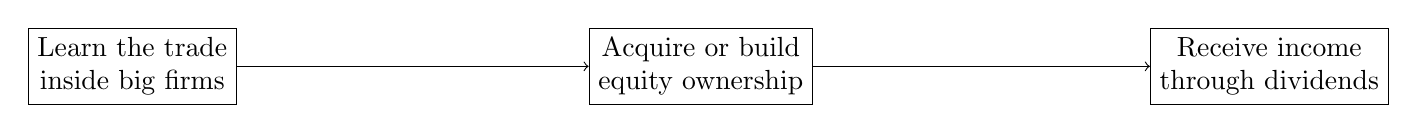
\begin{tikzpicture}[x=3.8cm,y=1.7cm]
\node[draw, rectangle, align=center] (a) at (0,0) {Learn the trade\\inside big firms};
\node[draw, rectangle, align=center] (b) at (1.9,0) {Acquire or build\\equity ownership};
\node[draw, rectangle, align=center] (c) at (3.8,0) {Receive income\\through dividends};
\draw[->] (a) -- (b);
\draw[->] (b) -- (c);
\end{tikzpicture}
\caption{A transcript-derived mobility sequence: apprenticeship produces competence, competence supports ownership, and ownership opens the channel from salary to dividends.}
\end{figure}

This figure is justified by the lecture's own narrative about family trajectory. The consultant says he came from nothing, learned his trade during roughly ten years in large firms, and then spent the next twenty to twenty-five years building his own companies. The lecture does not present that as a universal recipe, but it does present it as a repeated social pattern: apprenticeship first, ownership later.

When pressed for a lesson about entrepreneurship, he then gives the harsher formulation: most fail, so one needs a ``burn the ships'' mentality. Again, we should not dress this up as a theorem. It is motivational language. But the structural content is clear: commitment is being treated as the mechanism that keeps the entrepreneur from dispersing effort before the business can compound.

\section{Restaurants, Leadership, Household Support, and Real Estate}

The next major case turns to restaurants. At first it seems lighter, but in fact it changes the argument. The speaker says he bought a franchise so that someone else could do the heavy thinking while he ran the restaurants, and he also notes that he ran TGI Fridays as a chief executive. Leadership, not product novelty, becomes the center of gravity. Asked where people go wrong, he answers that they do not build a team that supports them, and they imagine themselves to be king.

This is a useful correction to the previous entrepreneurial sections. Ownership is not sufficient. Scale requires a surrounding structure of competent people, and leaders fail when they treat the organization as a mirror of themselves rather than as a coordinated system.

\subsection{Question \& Answer}

\paragraph{Question.} Is it always better to own the business yourself?

\paragraph{Answer.} Not necessarily. Ownership offers upside, but it also concentrates downside.

This interviewee gives the most explicit downside language in the lecture. If you own the business, you may have to put up your house and your assets. If you work for someone else, the downside is more limited: lose the job, then find another.

Let \(L(\mathcal{O})\) denote downside exposure in the owner state and \(L(\mathcal{E})\) downside exposure in the employee state. Then the transcript supports the qualitative inequality
\begin{equation}
L(\mathcal{O}) > L(\mathcal{E}).
\end{equation}

This is not a universal law of careers. It is the interviewee's way of naming the risk concentration attached to ownership. It also serves as a counterweight to the previous sections. Earlier, the lecture emphasized the power of equity. Here it emphasizes the burden of pledged collateral and concentrated exposure.

The same interview then pushes the analysis away from the firm and into the household. The speaker says bluntly that one must have support at home. If home life is miserable, work life and health deteriorate. That observation belongs in the chapter because it broadens the system boundary. The lecture is not pretending that wealth is produced by business decisions alone; it also depends on whether the rest of life stabilizes or sabotages the operating core.

Asked how to become a millionaire in 2024, this speaker says he goes long on real estate and even adds that real estate never goes down. We should preserve the force of the claim without turning it into doctrine.

\begin{remark}
The statement that ``real estate never goes down'' is best read here as interview testimony, not as a theorem of markets. The more careful part of the argument comes immediately afterward: the people who really made money owned the properties and the land rather than merely leasing and renting.
\end{remark}

The lecture then briefly breaks for a community announcement. Structurally, that interruption should not be mistaken for new analysis. It functions as a pause in the narrative before the final and most synthetic case.

\section{Self-Investment, Ruin, Recovery, and Cash Optionality}

The closing case begins with the visible luxury object that had been teased at the start: the Rolls Royce. The speaker says he is an entrepreneur, that he has been a business owner for \(25\) years after serving eight years in the Marines, and that his top-line revenue reached roughly \(40\) million. But once again the lecture quickly moves away from spectacle and toward mechanism.

The best financial advice he reports receiving came from a Goldman Sachs conversation. He had asked when \(10\) million could become \(20\) million. The reply, as he recounts it, was that someone like him was better off investing back into himself and his own business. The lecture then explicates that phrase carefully: skills, associations, relationships, reputation. This is a strong closing move. Wealth is not being treated as something that sits passively outside the person; it is being treated as something that can be re-planted into capacity.

The next pivot is even more important. He says he became a millionaire in his thirties, lost it in a bad relationship, and rebuilt it in his forties. Now the lecture raises one of its deepest conceptual tensions: what does one do after collapse? The answer comes in two layers. First there is a spiritual interpretation: when one is in the worst position, one is in the best position to hear a call one had ignored before. Second there is a practical interpretation: ruin strips away illusion and forces humility.

That humility reappears in the final ``billionaire'' lesson. What do billionaires do differently? They ask more questions, and they enter rooms without assuming they already know everything. The lecture thus turns its own interviewing style into part of the content. Curiosity is not only how the episode is made; it is also one of the habits said to separate the very wealthy from everyone else.

\subsection{Question \& Answer}

\paragraph{Question.} How does a downturn become an opportunity rather than a catastrophe?

\paragraph{Answer.} Only if one arrives at the downturn with liquid reserves.

The final advice about affording a Rolls Royce in \(2024\) is actually a miniature lecture on optionality. When interest rates rise and people who did not save are squeezed, assets that once sold at a premium can be forced into discount. Let \(P_{\mathrm{peak}}\) be the earlier, easier-market price and let \(P_{\mathrm{distress}}\) be the forced-sale price. The transcript suggests a discount range of roughly \(20\%\) to \(50\%\), so we may write
\begin{equation}
P_{\mathrm{distress}} = (1-\delta)P_{\mathrm{peak}},
\qquad
0.2 \lesssim \delta \lesssim 0.5.
\end{equation}

If we let \(M_t\) denote reserves accumulated during the good period, then the lecture's guiding implication is
\begin{equation}
M_t \uparrow \quad \Longrightarrow \quad O_t \uparrow,
\end{equation}
where \(O_t\) denotes purchase optionality when other holders must sell.

We can make the update rule explicit:
\begin{equation}
M_{t+1} = M_t + s_t,
\end{equation}
where \(s_t\) is the deliberate saving flow during favorable periods. The lecture's slogan is simple: in good times, stack cash; in stressed times, deploy cash.

A worked example makes the point concrete. If a luxury car was worth
\[
P_{\mathrm{peak}} = 500{,}000
\]
in the easier market, and if forced selling produces a \(30\%\) discount so that \(\delta=0.3\), then
\begin{equation}
P_{\mathrm{distress}} = (1-0.3)\cdot 500{,}000 = 350{,}000.
\end{equation}
The lesson is not really about cars. The car is just the local embodiment of a broader rule: liquidity has option value precisely when other people need immediacy more than they need price.

By ending on this point, the lecture quietly gathers many of its earlier strands into one place. Cash flow keeps the firm alive. Equity converts success into ownership income. Control must not be surrendered blindly. And saved cash turns bad times into purchase windows.

\section{Summary}

The lecture never presents itself as a formal theory of wealth, but a theory does emerge if we track the repeated mechanisms carefully. First, revenue is not enough; what matters is the cash-flow path and the capital buffer that the path preserves or destroys. Second, ownership changes the category of income: salary and bonus may pay well, but dividends tied to equity are what make the large jump. Third, financing is also governance; the money one accepts changes who commands the enterprise. Fourth, downturns do not create opportunity for everyone equally. They create it for those who saved before the stress arrived.

In short, the Dallas interviews reduce to a small but serious set of rules. Learn a trade well enough to own the upside. Keep a tight grip on cash flow. Be careful what sort of capital you invite in. Build teams and households that do not sabotage the operating core. And when the cycle turns, let liquidity do what rhetoric cannot: buy time, buy assets, and buy asymmetry.